\section{超伝導回路の大規模化}
    本研究の目的は共振器間の高強度結合素子の開発である。まずはこの研究のモチベーションについて説明することから始める。
    序章でも述べたが超伝導量子回路の集積度は年々向上しており、知名度の高い企業が研究開発に乗り出していることからも世間からの注目度は非常に高い。しかしながら、各々の量子ビットを効率よく相互作用させようとする際にはまだまだ課題も多い。超伝導量子回路を用いた大規模な集積回路として有名なのはD-wave社の量子アニーリング回路、Googleの万能型量子回路であるがその2つの例を見ても各々の量子ビットの全結合は実現できていない。量子ビットと結合素子を直接結合させるには回路デザインの観点から限界が生じている。我々の研究チームでは量子アニーリング型及び万能型のそれぞれについて2次元回路アーキテクチャの開発に取り組んでいる。この2つのアーキテクチャのうち特に量子アニーリング回路では本稿のテーマである。共振器間の高強度結合素子の開発が要となる。以下に大規模アニーリング回路を駆動するために必要なここの超伝導素子のパラメータを示す。

    この図には量子ビット間の実質的な結合強度Jijと量子ビットのパラメータが示されている。量子アニーリングはイジンぐモデルを前提に構築されたモデルであり、最終的な解は結合強度Jijにマッピングされる。始状態のパラメータは量子ビットの遷移周波数にマップされるため始状態と終状態において、この2つのパラメータはバランスがとれていることが前提となる。またスイープ時間において突発的な状態遷移を避けるために量子ビットの遷移周波数はGHz帯に設定する必要がある。この状況においてJijの強度をGHz体に保つためには共振器間の結合強度の絶対値には少なくとも400MHzが必要とされる。マッピングの自由度を上げるにはこのJijは正負でのバランスがとれていることが望ましい。
    以上より共振器間の結合に要請される理想的なパラメータは-400MHzから400MHzを自由に変調できるものである。
    先行研究\cite*{Wulschner2016}では-320MHzから37MHzの結合強度を実現しているが、正負両方向において強度不足であることがわかる。

\section{}

\section{結合振動子}
    本研究のテーマはエンジニアリングな側面が強いが、研究対象としている結合共振回路は物理モデルとしても非常に興味深い内容である。量子力学と古典力学のアナロジーとして連成振動子モデルは多くの研究がなされている。\cite*{Rodriguez2016}\cite*{Ivakhnenko2018}\cite*{Novotny2010}
    上記のモデルは一般的な共振素子(振動子)と共振素子を結合した系を理論的視点から論じている。今回作成した共振回路は共振器間のダイレクトな結合強度を変調できるという点で非常に魅力的である。一般的な共振素子はその遷移周波数がすべて同一であり、共振回路の周波数を持った光子を外部から入力しても高準位へと遷移してしまい、光子の放出現象は示さない。しかし、振動子間に結合項が存在すると振る舞いは一変し新たな固有モードが出現する。古典力学ではしばしばこのモードのことを基準モードと呼んでいる。この
    \begin{figure}[H]
        \centering
        \includegraphics[width=9cm]{b.pdf}
        \caption{エネルギースペクトル}
    \end{figure}
    \begin{figure}[H]
        \centering
        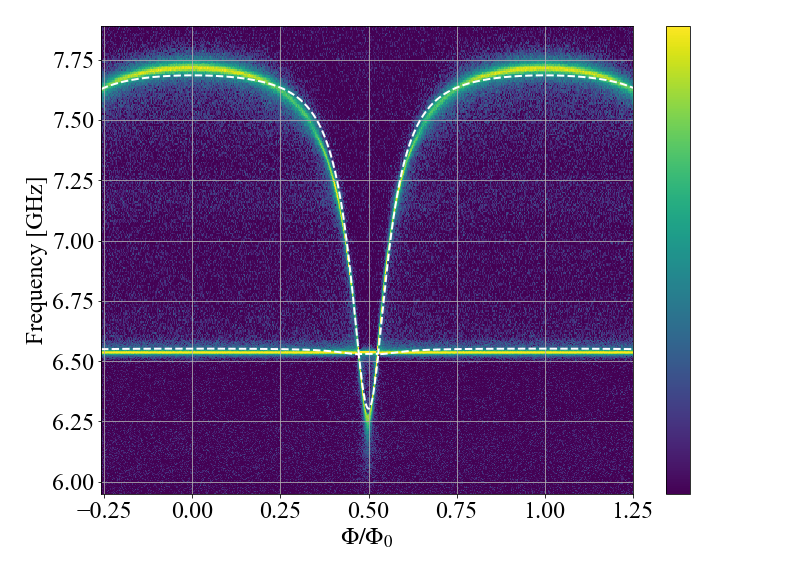
\includegraphics[width=9cm]{a.png}
        \caption{エネルギースペクトル}
    \end{figure}
    \begin{figure}[H]
        \centering
        \includegraphics[width=9cm]{c.pdf}
        \caption{エネルギースペクトル}
    \end{figure}


